\documentclass[../main.tex]{subfiles}


\begin{document}
\raggedright

To begin with, the extenuating circumstances page\cite{ecfuni} will have a link to take the student to the new website portal which will contain a login page allowing the student to login with his or her university email. Once the student has logged in, an option to start a new extenuating circumstance form will be displayed and clicking on that the student will be presented with a form to fill online. Once the online form is filled with all the details it will be stored on their profile and displayed on the "Dashboard" of the portal. The same form can then be accessed over time with new feedback, approval and other statuses. Any updates by the scrutiny committee will be notified to the student via email. \\[2mm]


The portal will also allow the scrutiny committee to login and control the movement of the forms as well as provide feedback and comments to the student regarding their circumstance. They will also be able to request more proof and evidence if need be. The forms can then be processed further and exported as documents such as PDF's and TXT's allowing the relevant stakeholder to print or share. Figure~\ref{fig:portal1} describes the authentication and users process.

	\begin{figure}[H]
        \center{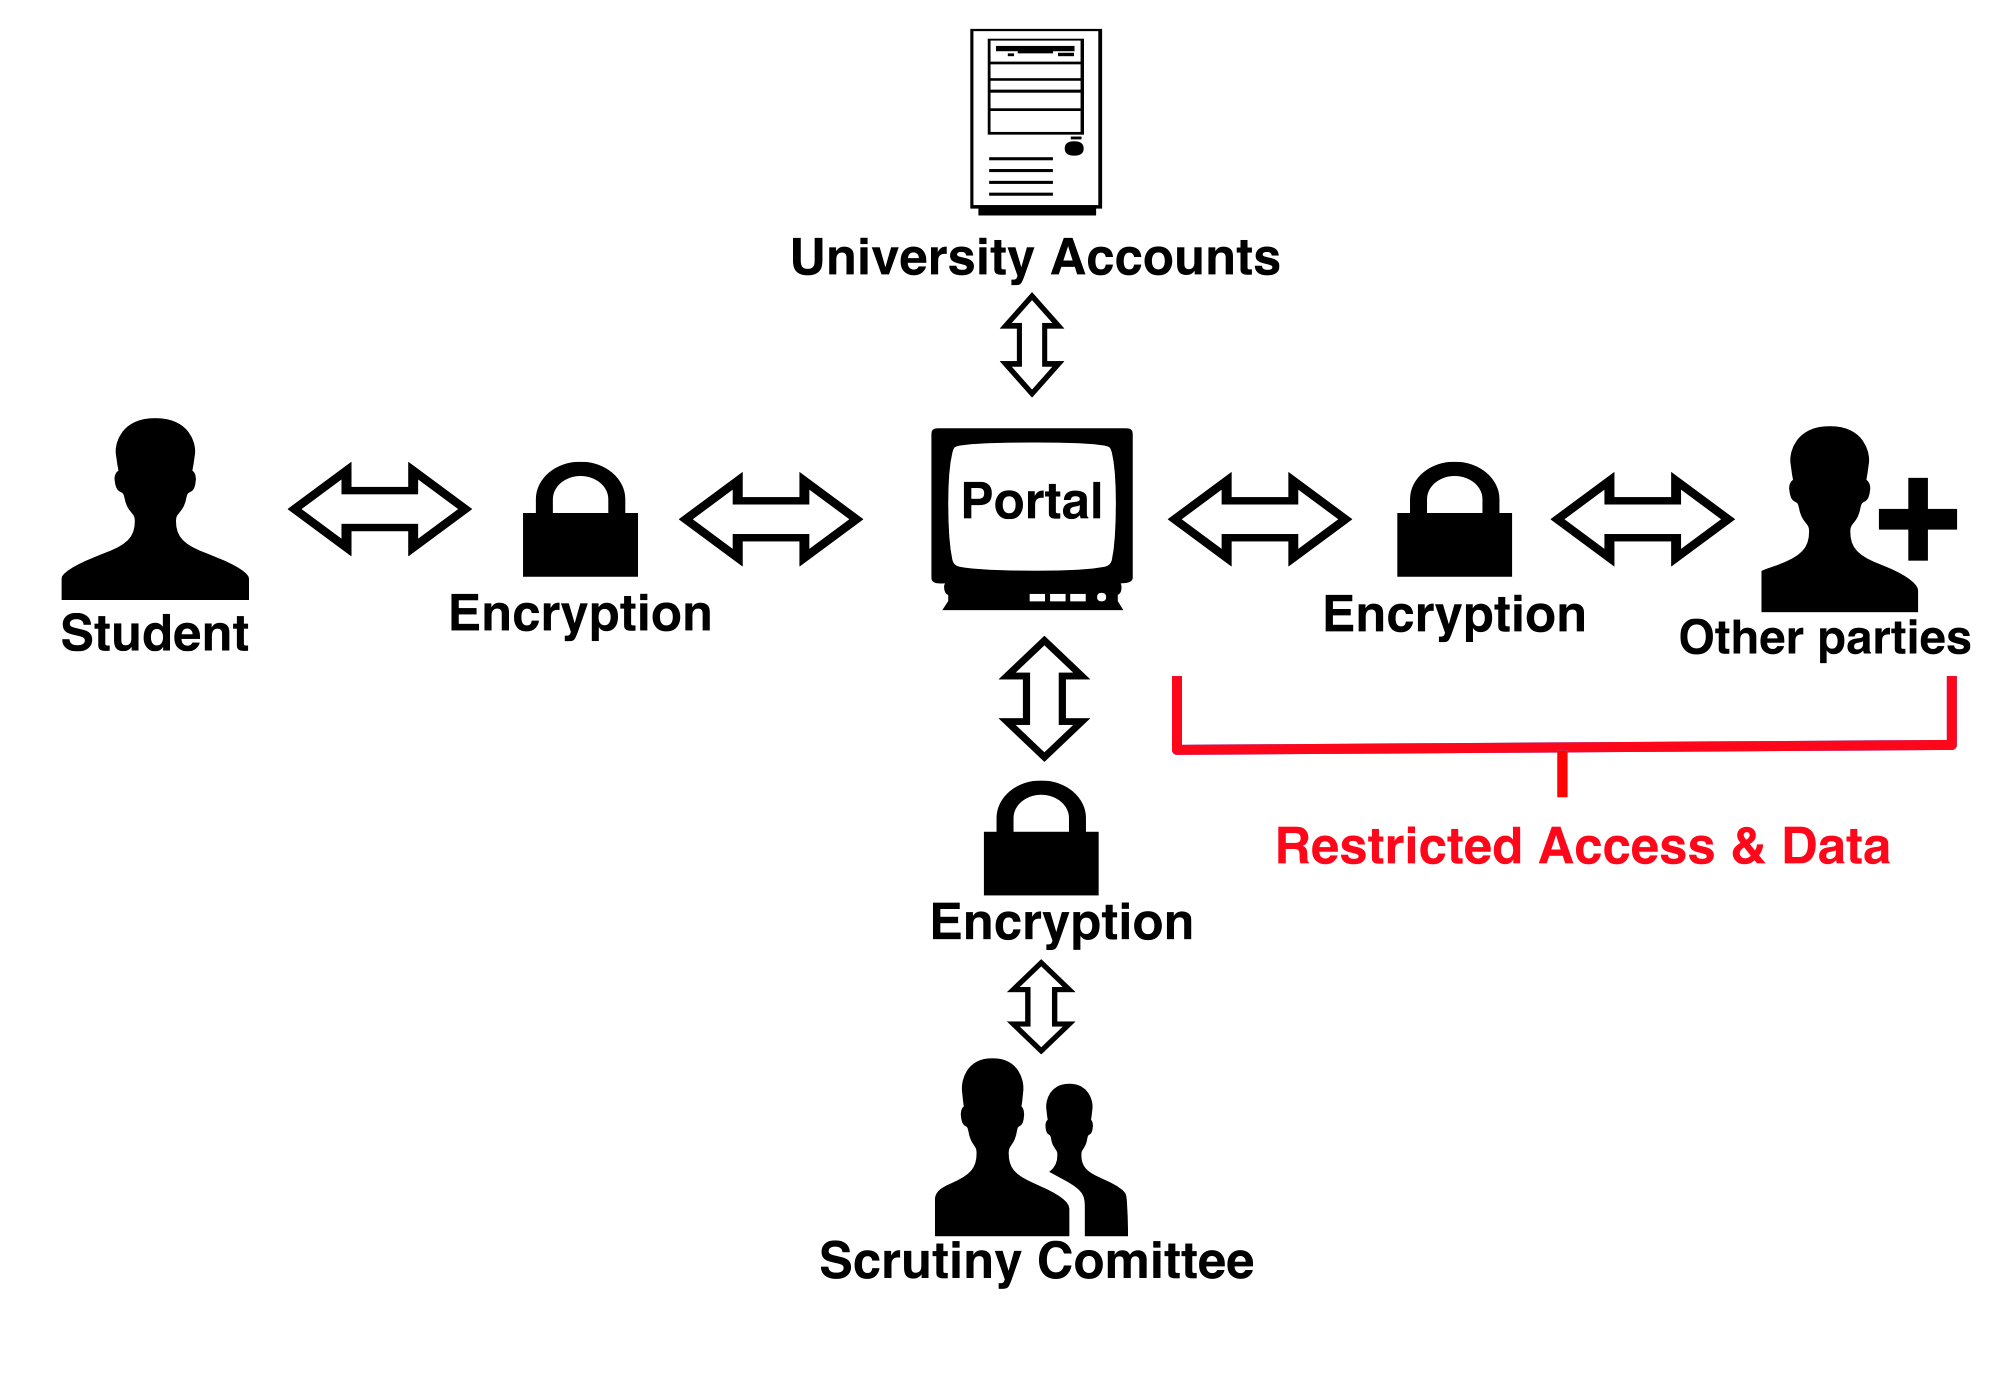
\includegraphics[scale=0.3]
        {images/portal1.png}}
        \caption{\label{fig:portal1} Portal and users.}
      \end{figure}

The web system will be entirely encrypted and data will be stored in a secure database as presented earlier in Figure~\ref{fig:basicwebdesign}. This allows total security of the information stored and only users with access will be allowed to get that information. Some users will be restricted such as the other parties who get the students condition without knowing exactly what it is they are having trouble with. This allows confidentiality while allowing access at the same time. 


\end{document}
